\section{Application to the COVID-19 outbreak}
\label{sec:covid}

The mathematical model described in Section~\ref{sec:model} is checked against data of the oubreak in Lombardy in  Figure~\ref{fig:data_lombardy}. \\

The dataset indicates only the total cases, corresponding to positive tested population, deaths and recovered people. In the model, this quantity is estimated by the sum of quarantined $Q$, deaths $D$ and recovered $R$ categories. The infected and exposed population is here not considered due to the testing campaign adopted in Lombardy. Only people with a chance of having contracted the virus (medical staff, people close to positive cases) and infected people developing heavy symptoms to need hospitalisation. Since exposed and infected categories contain individuals with the virus but with at most mild symptoms, they are not tested and are not included in the numbers of  positive  cases. The quarantined category contain people getting hospitalised and therefore being immediately quarantined by the medical structure. \\

Since the plateau of the total cases is not reached in data, the most important parameters to tune to agree with the collected data are $\beta$, $\braket{k}$, $\delta$ and $\tau$ parameters. On top of the parameters described in Section~\ref{sec:model}, an additional parameter $t_0$ has been added to shift the distribution in time. The  prediction that matches at most with data, after tuning the model parameters, is shown in Figure~\ref{fig:data_vs_model_first_lombardy}. Parameters modifying the trailing edge of the infection is set to approximate values of the outbreak. Mortality is set to $2\%$, reinfection probability to $10^{-5}$ since yet no cases have been observed. Population is set to $10^7$, corresponding to Lombardy population.\\

\begin{figure}
\centering
  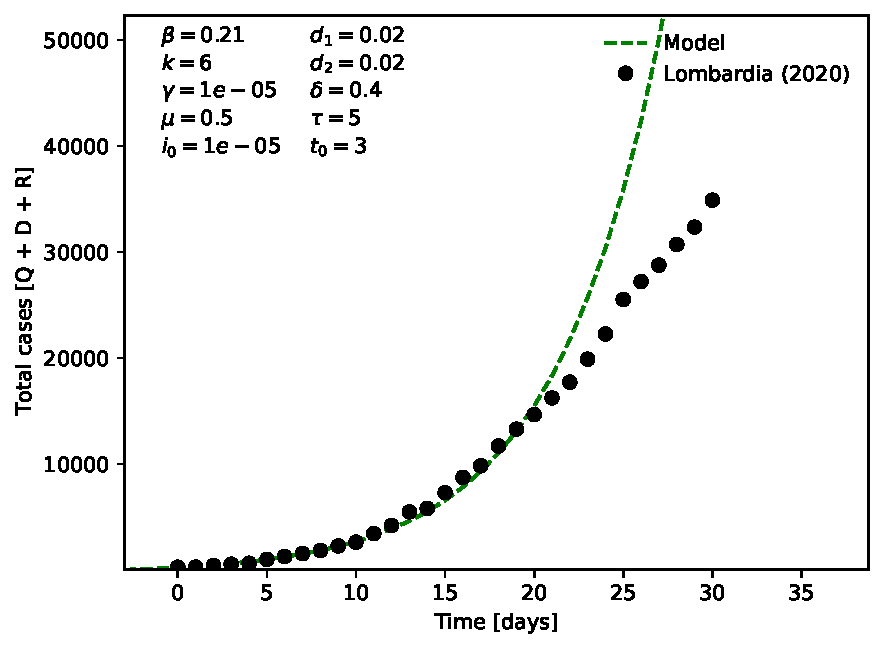
\includegraphics[width=0.4\textwidth]{imgs/Covid/DataVsModel_parameters_Lombardia_less_impacting.pdf}
  \caption{Best match of parameters to make the model described in Section~\ref{sec:model} fit with data il Lombardy.}
  \label{fig:data_vs_model_first_lombardy}
\end{figure}

As shown in Figure~\ref{fig:data_vs_model_first_lombardy} the model predicts an exponential growth until the peak, that is not what is measured, since different slopes of curve are present in data. The hypothesis is that the parameters of the model changes in time due to the several restrictions applied to social activity to contain the virus spreading  (non-essential activities closed, cancellations of events, etc.). These regulations cause a decrease of the total cases slope, impossible to predict with the mathematical implant of Section~\ref{sec:model}. \\

Two main measures to contain the virus have been introduced since March 1st, when the outbreak started to significantly spread. The first strong limitations have been introduced on March 9th \cite{DPCM-0903} and 11th \cite{DPCM-1103}, the so-called \emph{\#iorestoacasa} laws, forcing non-essential activities to close and encouraging home-quarantine. More stringent laws, prohibiting any movement outside the city of residence and forcing the lock-down except for emergencies, have been released on March 20th \cite{DPCM-2003} and 22th \cite{DPCM-2203}. This regulations are still valid at the time of writing (April 15th). Indeed, around those dates, the slopes of the total cases curves change, confirming that these procedures have been important to contain the spreading of the virus. The mathematical model described in Section~\ref{sec:model} is then modified to reflects these changes and to model better the data behaviour.

\subsection{Adapting the model to real-world scenario}
\label{ssec:impr_model}


To adapt the model to the real world scenario, few improvements have been implemented:
\begin{itemize}
\item Inclusion of a recovery rate for the infected category evolution.
\item Fluctuation of $\delta$ parameter: this reflects the fluctuation of the number of tests performed per day.
\item Scheduling of $\braket{k}$ parameter: this reflects the social-distancing measures.
\end{itemize}

A scheduling of the $\delta$ parameter is not introduced. This implies that the fraction of the infected people getting tested is almost constant over time. This assumption is reasonable since the testing strategy has been kept consistent over time. Indeed, the mortality rate, normalised by the number of tests, is quite flat.\\

The original model does not include a recovery rate for the infected category. Therefore an infected person is only expected to develop symptoms and get quarantined. A person heals only if quarantined before. This is not the real case, the infected people are identified as non-symptomatic contagious infected individuals, and they can recover from the virus without being hospitalised, tested and quarantined. Therefore the variation $\dot{i}$ is modified as follows:
\begin{equation}
\dot{i} (t)= \beta\braket{k}s(t-\tau)i(t-\tau) - d_1i(t) - \delta {i(t)} - \mu{i(t)}
\end{equation}
This part of recovered people are not counted in the recovered category.\\

Corrections of the $\delta$ parameter over time are derived to account for the non-constant rate of performed test and shown in Figure~\ref{fig:tests_vs_time}. A functional model has been fitted to the data points (taken from reference \cite{Lab24}) and the corrections are computed as ratio of the observed points with respect to the function. The function is consistent with the choice of a constant $\delta$ since it approximately describe the data trend in Figure~\ref{fig:data_lombardy}.\\

\begin{figure}
\centering
  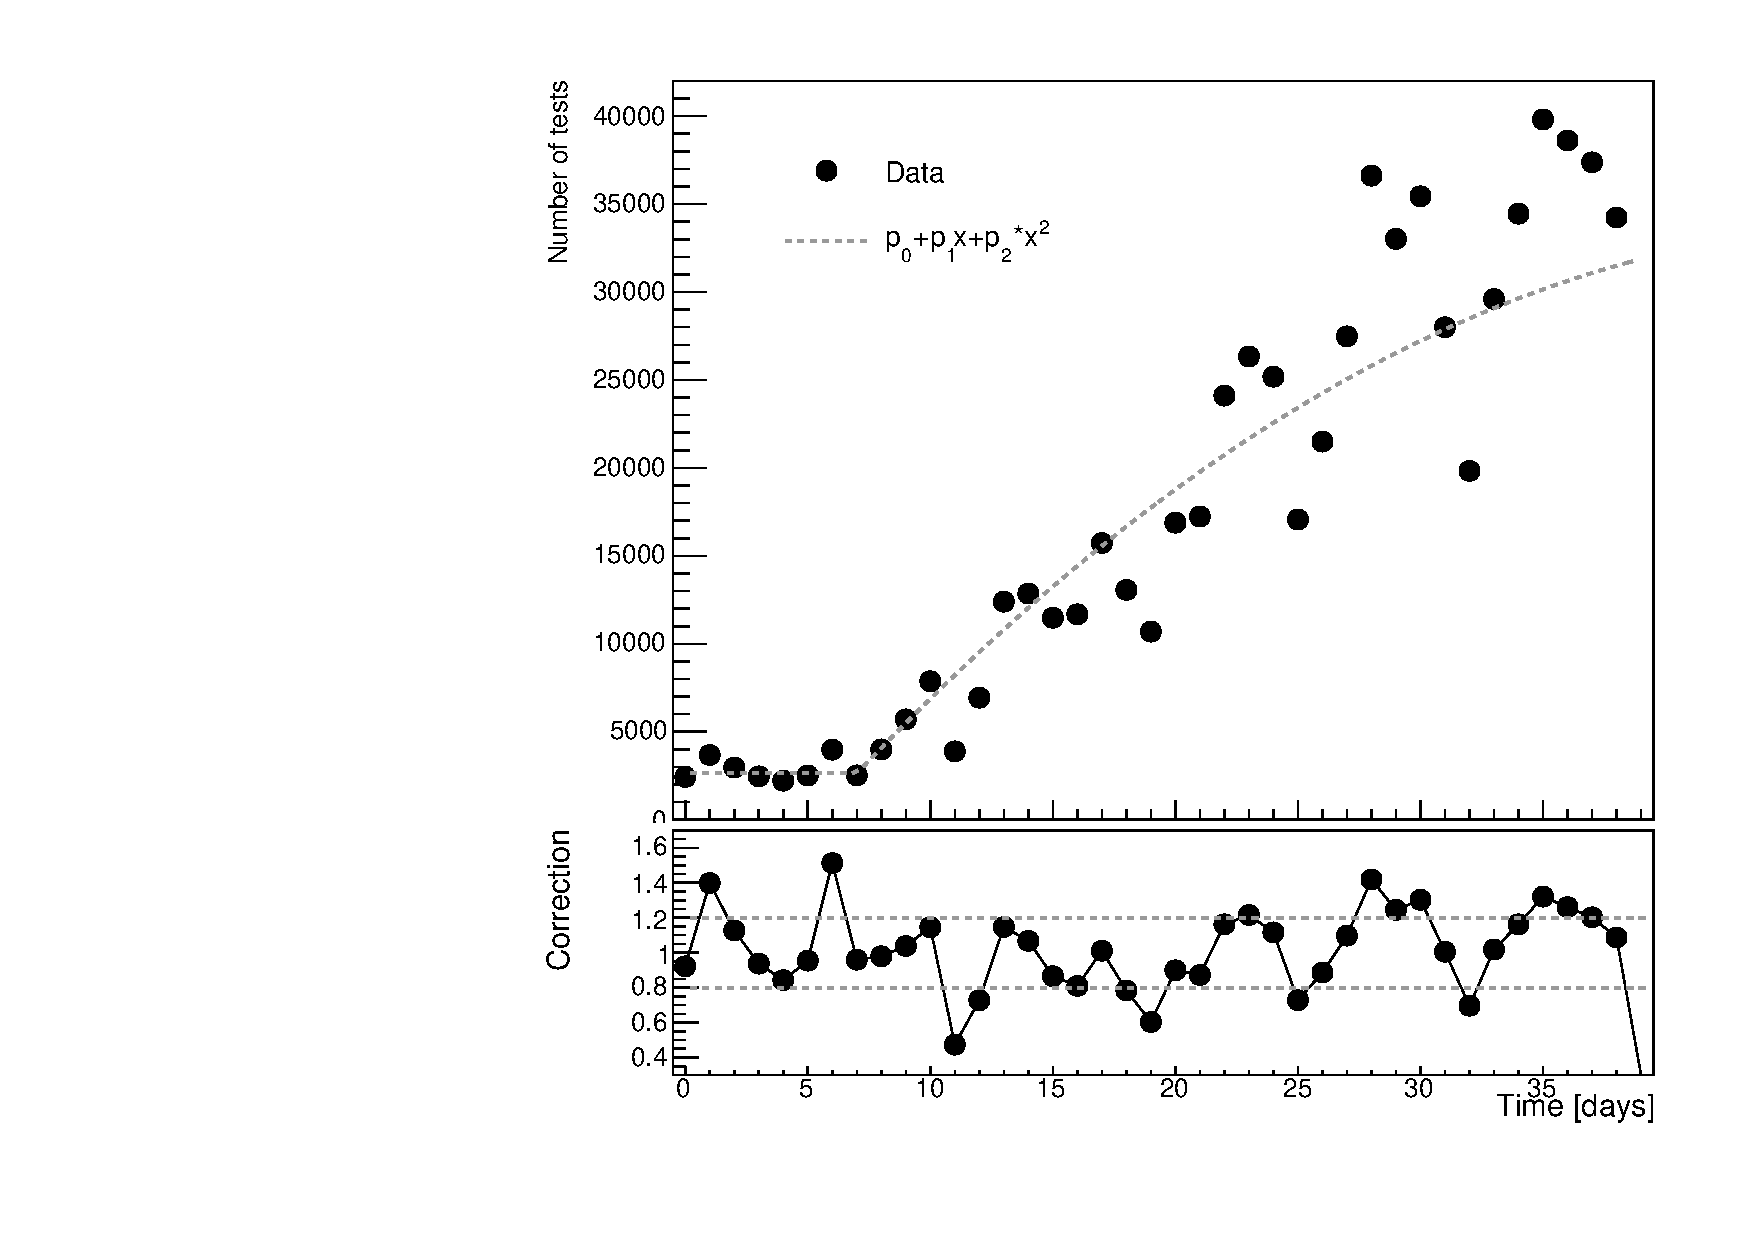
\includegraphics[width=0.4\textwidth]{imgs/Covid/TamponsCorrections.pdf}
  \caption{Numbers of performed tests over time in Italy. A constant plus a third degree polynominal is fitted and corrections (plot below) are extracted as a difference of the measured points to the functional model.}
  \label{fig:tests_vs_time}
\end{figure}

This correction is introduced to describe the non-smooth behaviour of the curve. However, since this data are available national-wise, the numbers for Lombardy may differ. This possible discrepancy is accounted in the fit, described in Section~\ref{ssec:plf}. \\

The $\braket{k}$ scheduling represents the introduction of social-distancing, varying from a freely-communicating system (where  $\braket{k}$ is set to the initial value) to the lock-down situation in which an infected person interact only with few susceptible individuals (family).\\

\begin{figure}
\centering
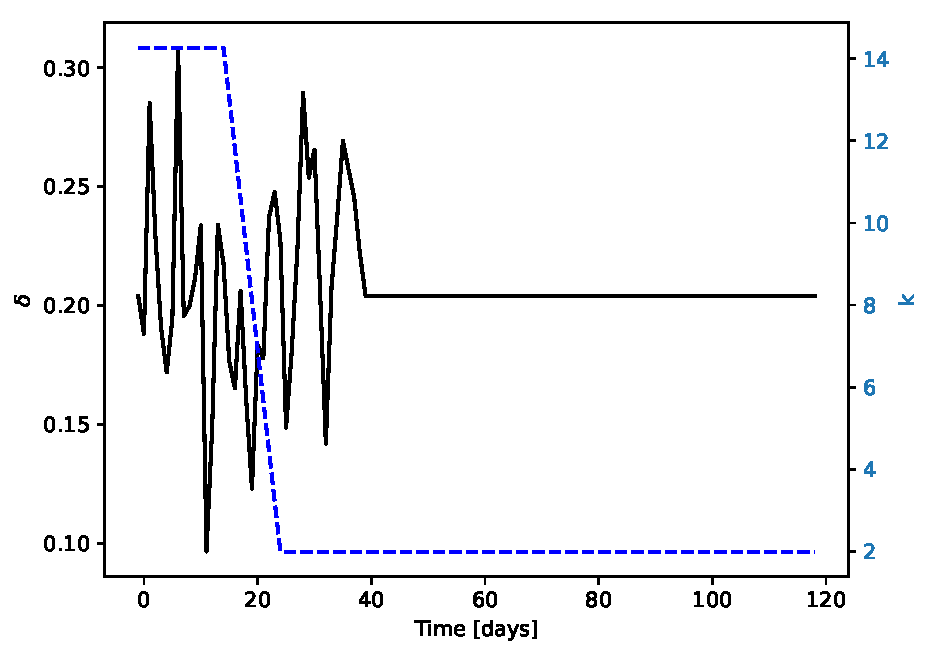
\includegraphics[width=0.4\textwidth]{imgs/Covid/Scheduling_regular.pdf} 
  \caption{Variations of $\delta$ and $\braket{k}$ parameters over time. The reference values of the parameters are set the same as in Figure~\ref{fig:data_vs_model_first_lombardy}.}
  \label{fig:scheduling}
\end{figure}

The values of $\delta$ and $\braket{k}$ parameters over time is shown in Figure~\ref{fig:scheduling}. A new set parameters is tuned to approximately match data shape. This new tuned prediction is shown in Figure~\ref{fig:model_vs_time}, while the comparison with data is presented in Figure~\ref{fig:model_vs_data}.\\

\begin{figure}
\centering
\subfloat[\label{fig:model_vs_time}]{ 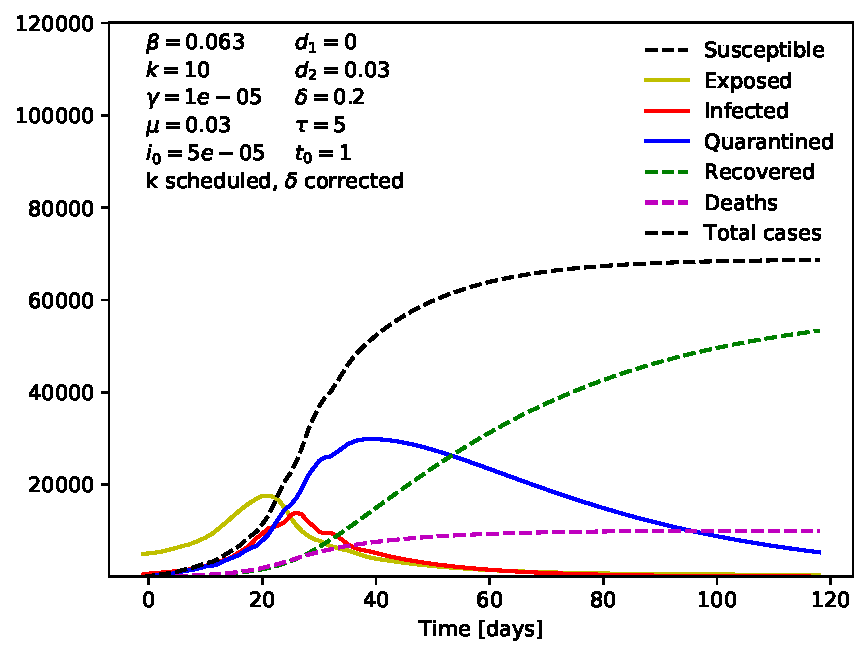
\includegraphics[width=0.4\textwidth]{imgs/Covid/Summary_parameters_Lombardia_scheduling_corrected_definitive_v2.pdf} }
\subfloat[\label{fig:model_vs_data}]{ 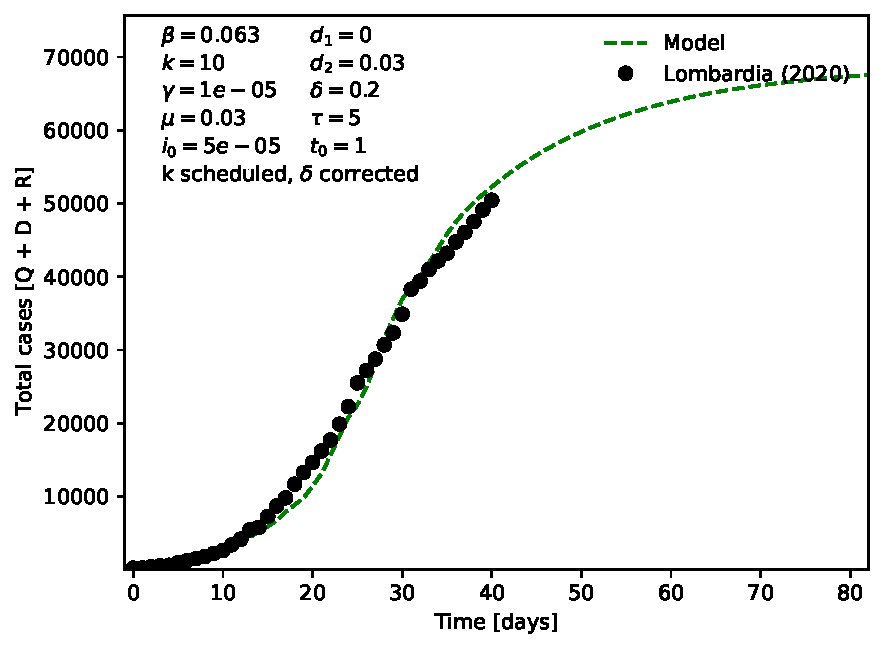
\includegraphics[width=0.4\textwidth]{imgs/Covid/DataVsModel_parameters_Lombardia_scheduling_corrected_definitive_v2.pdf} }
  \caption{Prediction of the improved model for the population classes with the correction with a new set of tuned parameters (a). Comparison of the model in (a) with the data collected in Lombardy (b).}
  
\end{figure}



\subsection{Profile likelihood fit to data}
\label{ssec:plf}

The model parameters are measured with a Profile Likelihood fit. The fit is performed using \textsc{ROOT} framework \cite{ROOT}, in particular with the \emph{HistFactory} framework to create statistical models \cite{HistFactory}.\\

The observable used in the fit is the daily number of total cases (deaths, quarantined and recovered) to use uncorrelated quantities for each bin of the fitted distribution. The distribuition is rebinned to increase statistics per bin. The Parameter of Interest (PoI) is a global normalisation factor of the distribution, introduced as a free floating parameter. This corresponds to a variation of the initial condition, $i_0$, that is not included in the set of parameters to fit. The profile likelihood fit adjusts the model parameters to maximise the likelihood of the data given the assumed model \cite{HistFactory}.\\
  
Since no functional model is available, templates of the total cases distribution for different choices of the model parameters are generated and used in the fit. For each parameter of the model, two templates of the distribution are generated, corresponding of increasing and decreasing of a $10\%$ the parameter value. A nuisance parameter (NP)of the model, with Normal Gaussian prior, is associated to each model parameter used in the fit. The variation of each template from the nominal predictions given by the variation of a single parameter is associated to the variation of the associated NP, whose $\pm1$ standard variation correspond to the two differences of the templeates in input. For middle values of the NP, an interpolation is used bin-by-bin, to get the corresponding effect of the parameter on the distribution. An example of the effect of the variation of a model parameter is shown in Figure~\ref{fig:alpha_beta}. To improve the fit stability the effect of the NPs are symmetrised against the nominal prediction. In case both variations are on one side, as in Figure~\ref{fig:syst_np}b, the variation is one-sided symmetrised.\\

\begin{figure}
\centering
\subfloat[\label{fig:alpha_beta}]{ 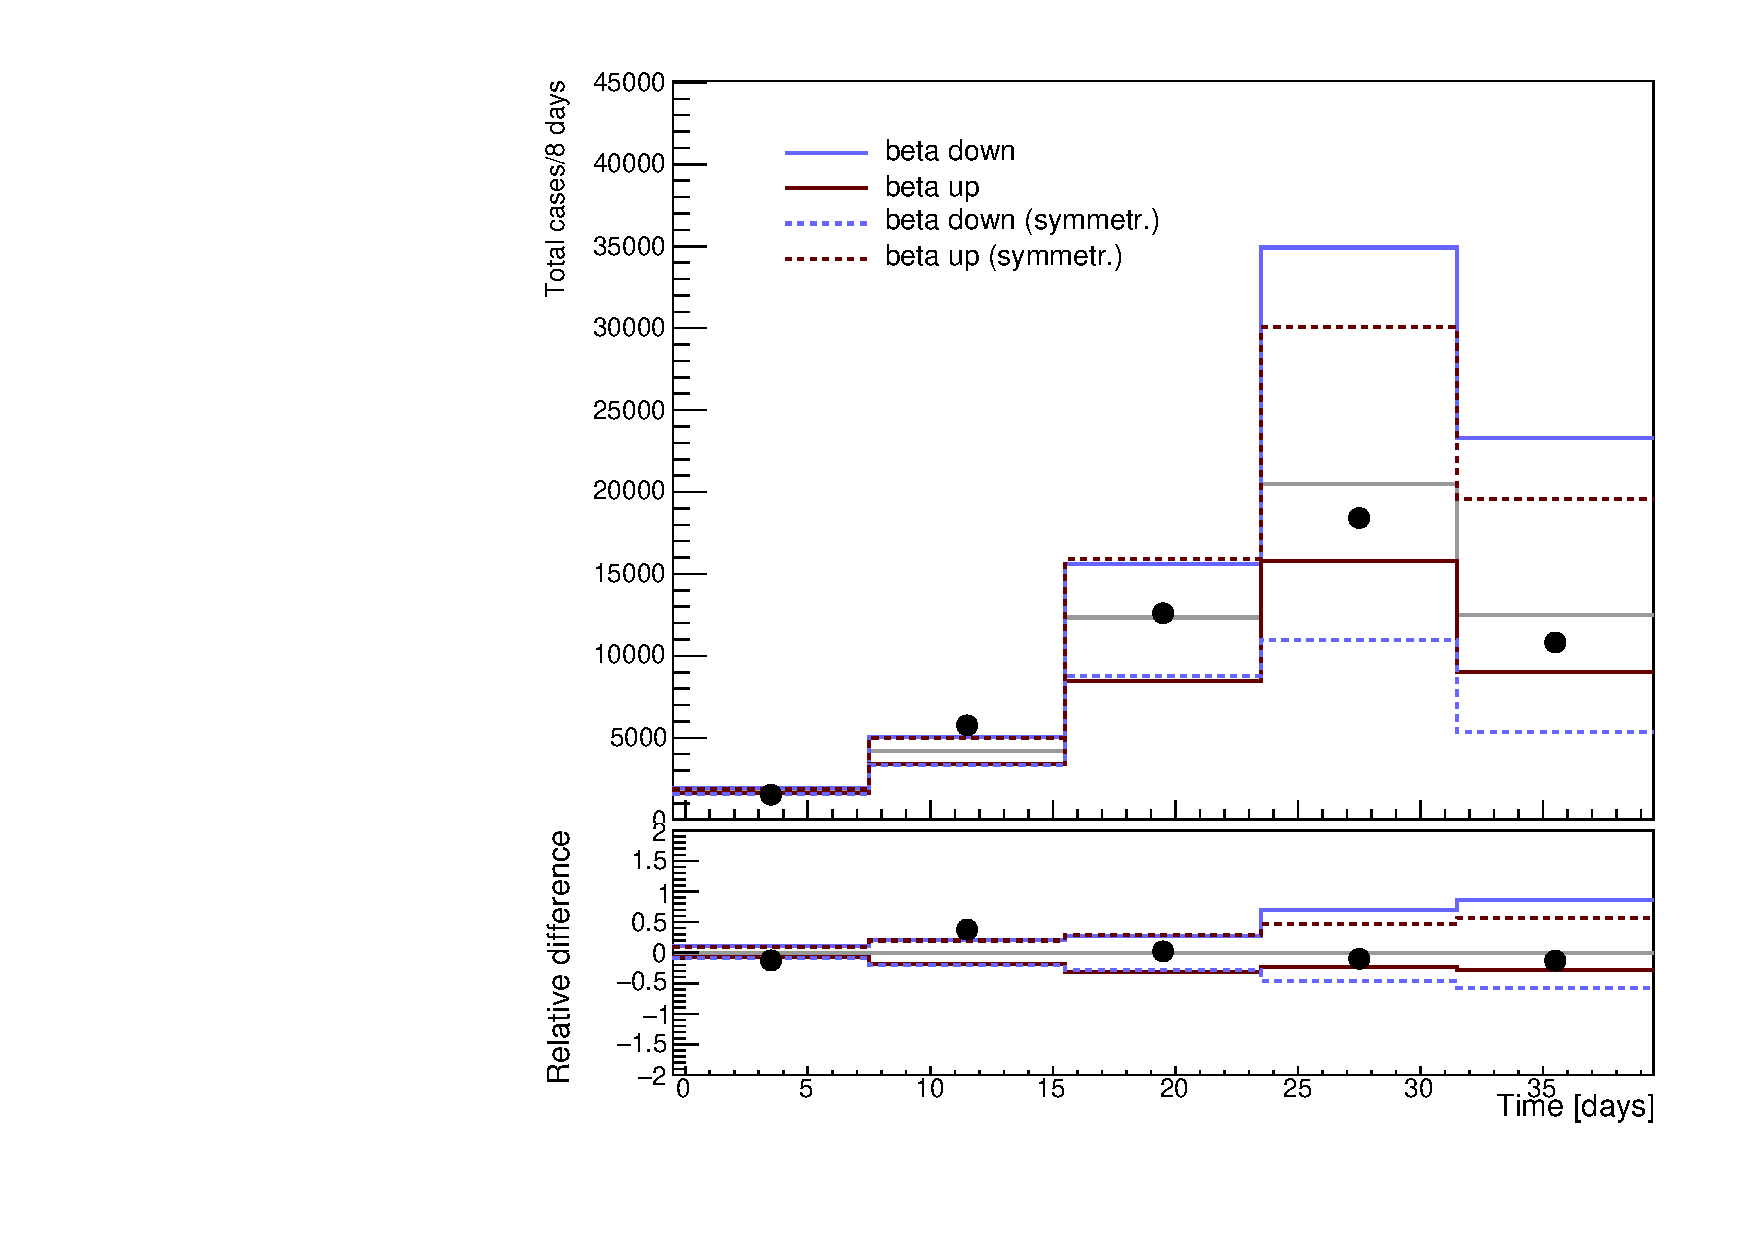
\includegraphics[width=0.4\textwidth]{imgs/Covid/Syst_beta.pdf} }
\subfloat[\label{fig:alpha_mu}]{ 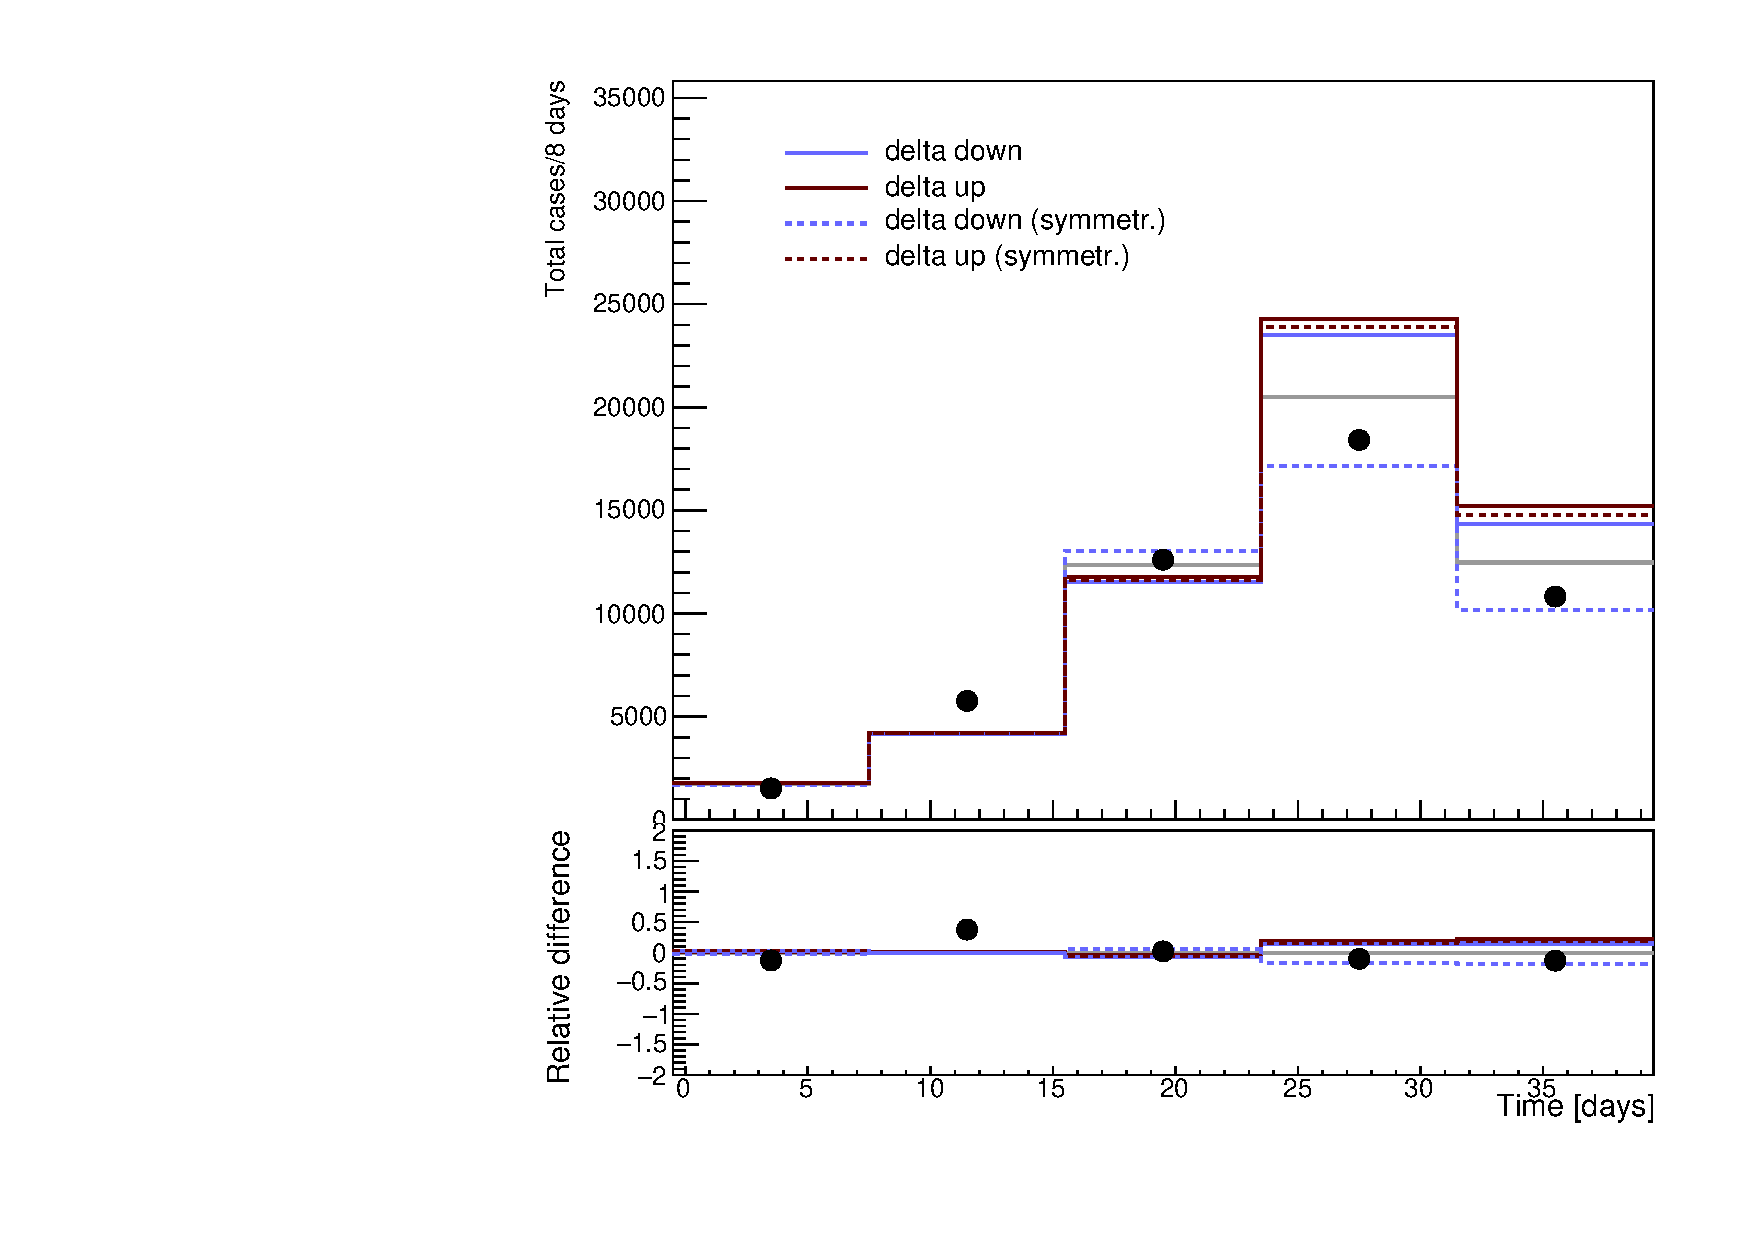
\includegraphics[width=0.4\textwidth]{imgs/Covid/Syst_delta.pdf} }
  \caption{Two examples of NPs included in the fit: variation of $\beta$ (a) and $\delta$ (b) parameters. In the $\delta$ parameter case, a one direction effect of the parameter is expected. A higher value of $\delta$ increases the number of quarantined people per day.  A lower value of $\delta$ instead makes the spreading faster, increasing the number of infected and then of quarantined people as well. In both plots the effect of the symmetrised variation is shown.}
  \label{fig:syst_np}
\end{figure}

To give enough degrees of freedom to the fit, additional NPs are used to take into account uncertainties on the $\delta$ correction described in Section~\ref{ssec:impr_model}. From Figure~\ref{fig:tests_vs_time}, a variance of $20\%$ is estimated, and a NP for each bin is added, assuming that the variations are uncorrelated bin-by-bin. The example for the two highest bins are shown in Figure~\ref{fig:syst_np_corrbin}.\\

\begin{figure}
\centering
\subfloat[]{ 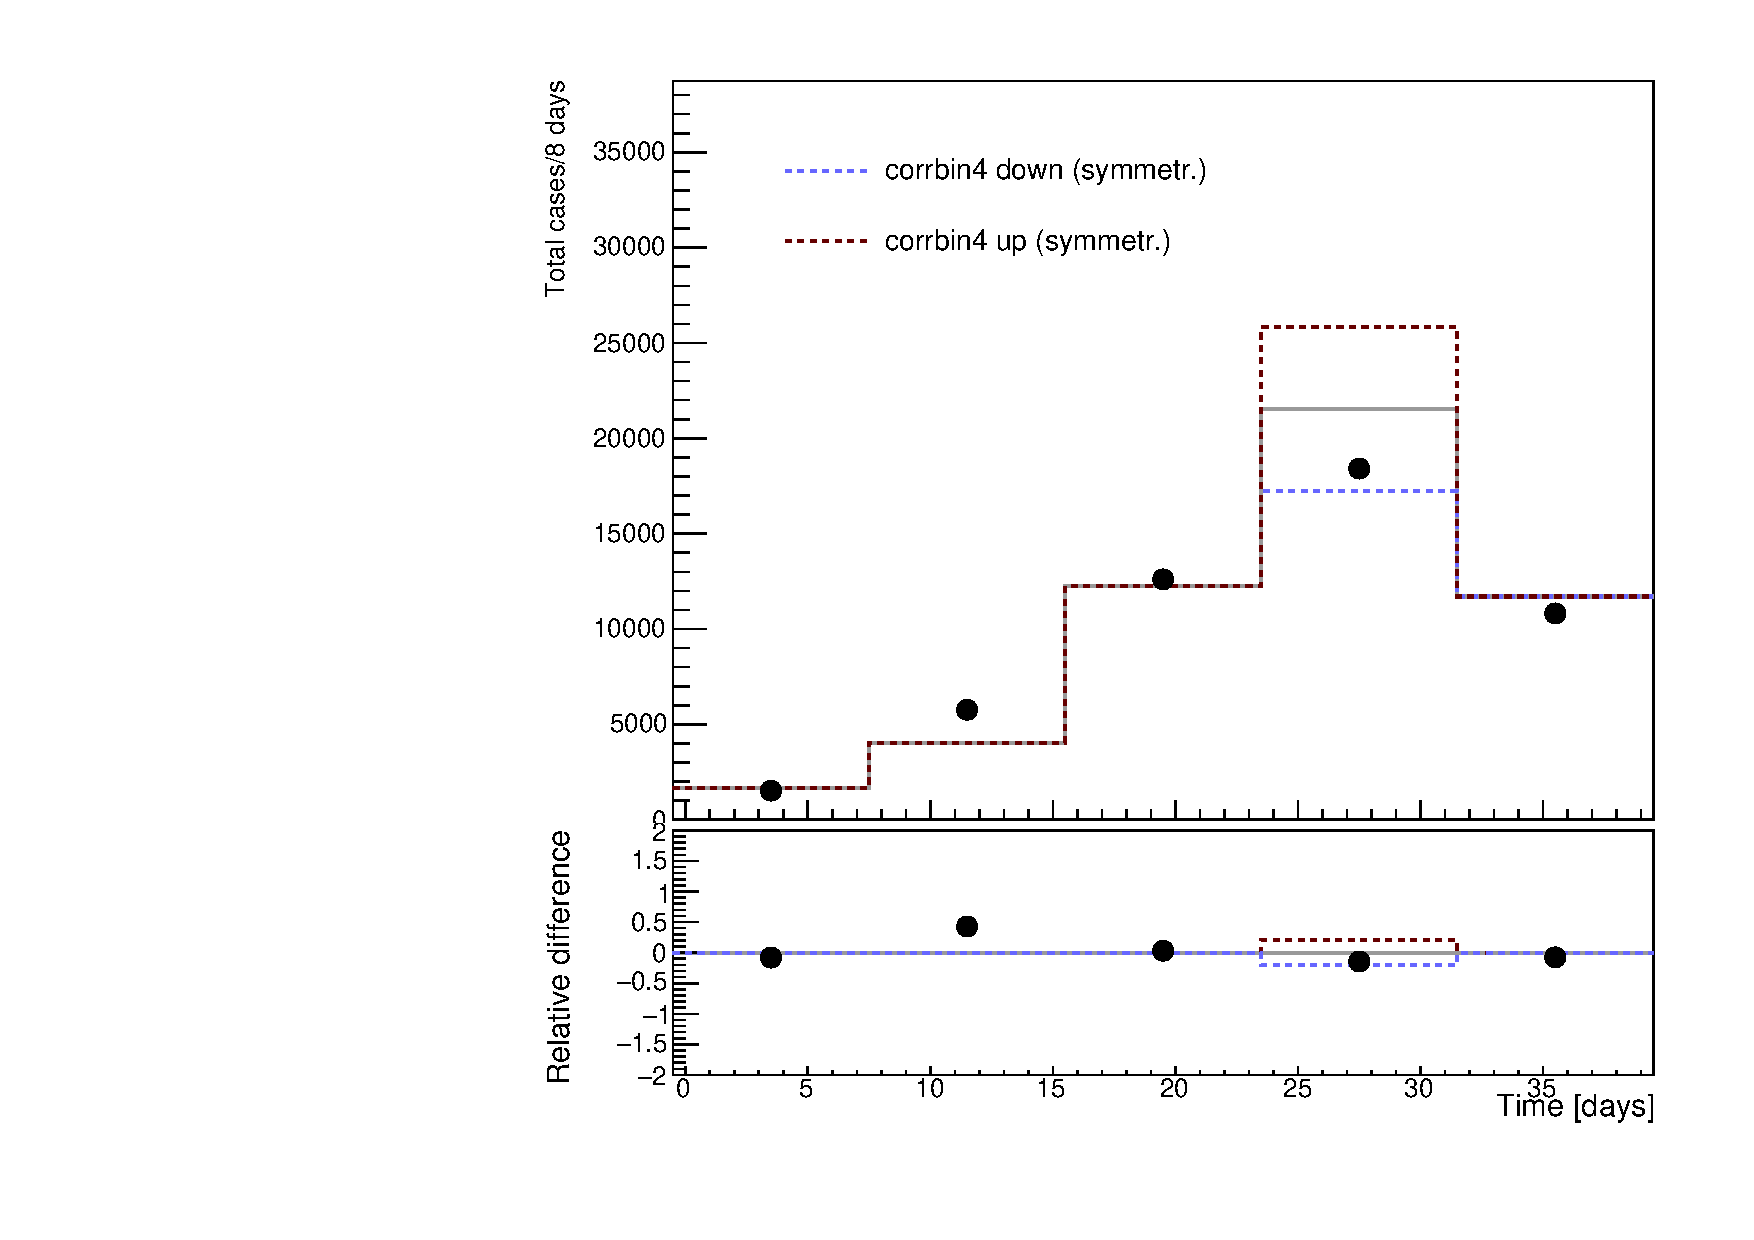
\includegraphics[width=0.4\textwidth]{imgs/Covid/Syst_corrbin4.pdf} }
\subfloat[]{ 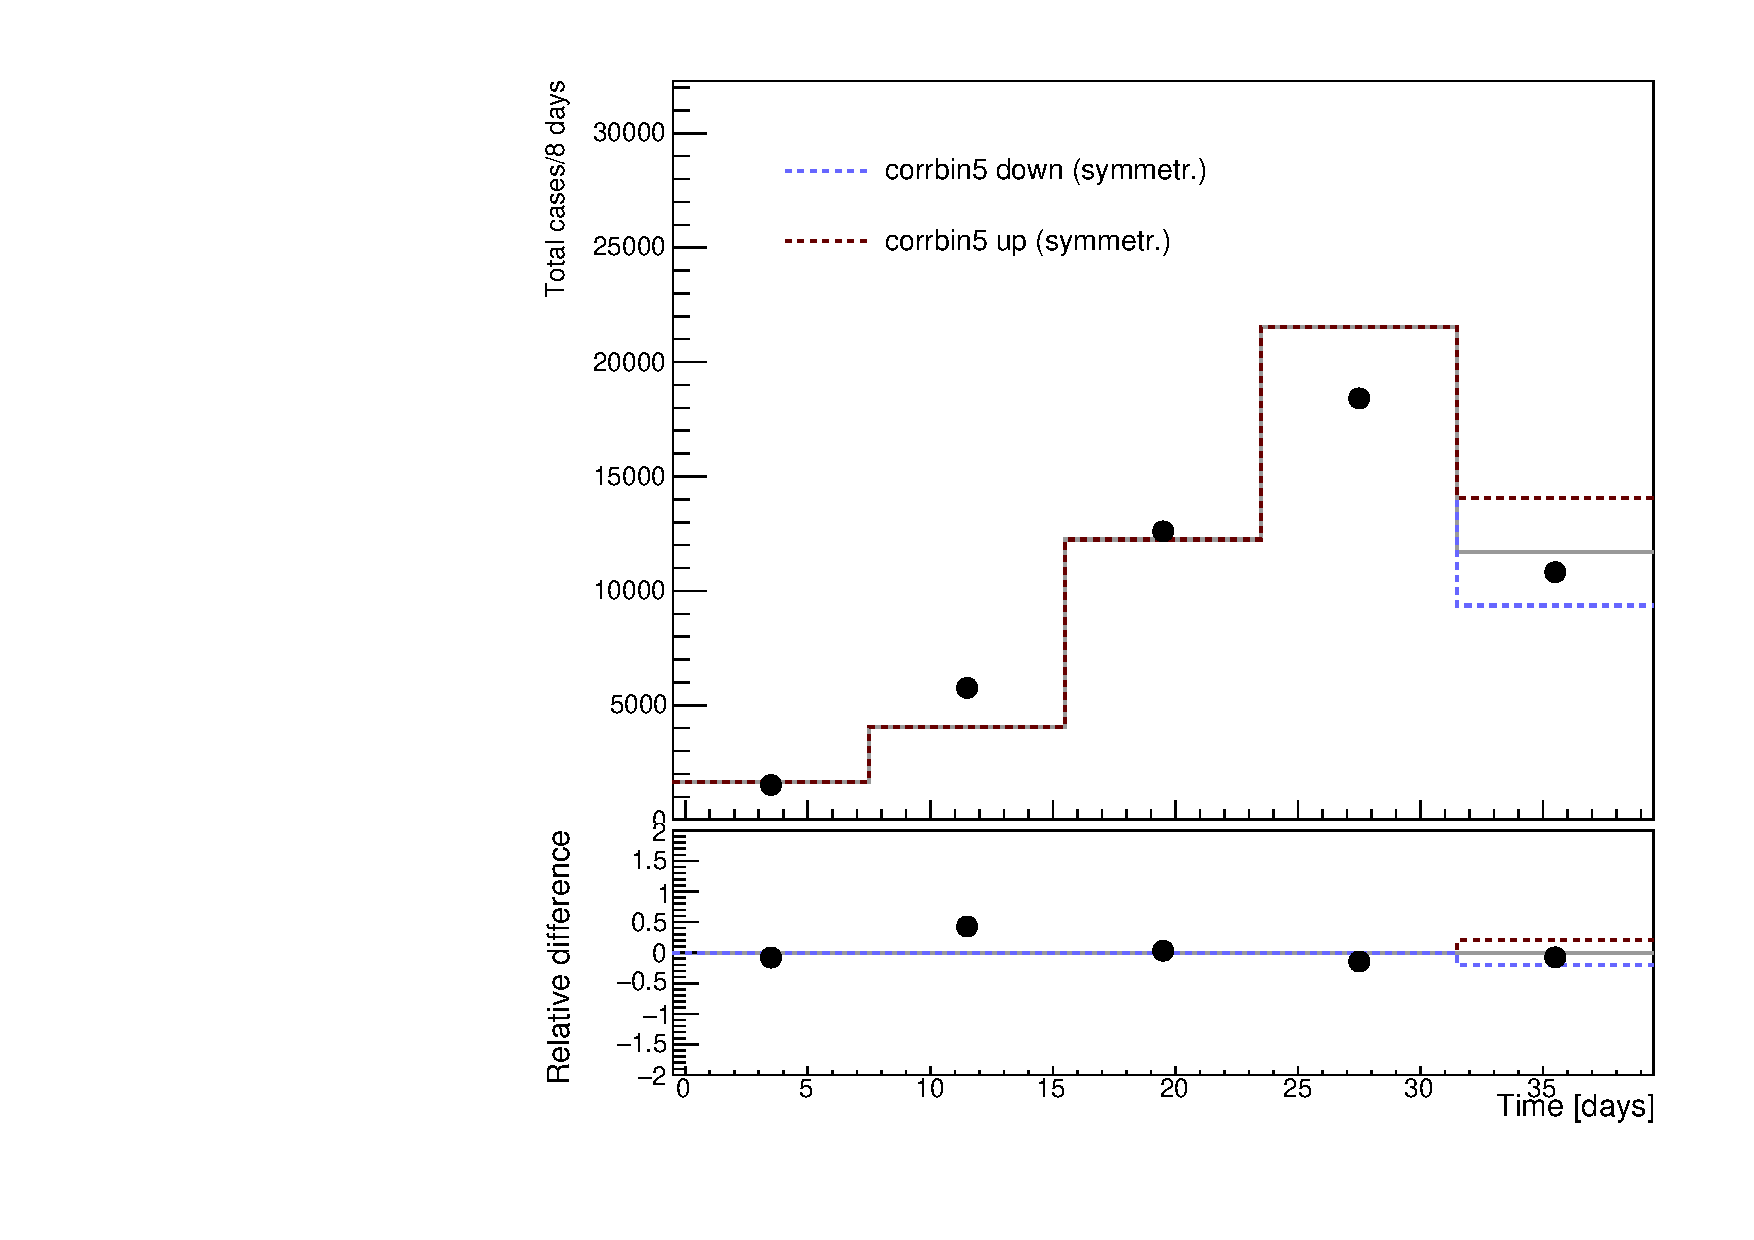
\includegraphics[width=0.4\textwidth]{imgs/Covid/Syst_corrbin5.pdf} }
  \caption{Variations associated to the test-based $\delta$ parameter corrections on the most significant bins in terms of the shape of the outbreak spreading.}
  \label{fig:syst_np_corrbin}
\end{figure}

The pre-fit prediction is shown in Figure~\ref{fig:prefit}, showing a good agreement of the data with the model withing the (large) uncertainties. The summary of the fitted model parameters and their correlations are shown in Figure~\ref{fig:nps}. Figure~\ref{fig:nps}a shows the pre-fit NPs value, equal to zero, following a Normal Gaussian distribution. The points indicate the post-fit values and associated uncertainties. The uncertainties on the parameters are constrained, meaning that the assumed systematics model is conservative and the NPs are measured with a higher precision than the assumptions. This is acceptable, since the used $10\%$ uncertainty on the parameters is set arbitrarily, choosing the smallest uncertainty range for all the parameters that cover the discrepancies of the model with data. Large pulls, over one standard deviations are observed in just two NPs, corresponding to the correcions on the bin contents. This is acceptable as well since the  uncertainty on those two parameters are estimated assuming the Gaussian fluctuations on the fitted model in Figure~\ref{fig:tests_vs_time}. In case the Lombardy tests are way different from the coutry-wise data in some periods, this assumption is not valid and pulls may appear. The parameter of interest, denoted as \emph{SF}, is expected to be unitary and still fitted consistently to the expectaion within one standard deviation. Correlations between parameters are understood: the scale factor, $\beta$, $\tau$ and the bin corrections are the most correlated, since they are the most important parameter to change the distribution shape in the fit range. The correlations are coherent with the expectations since they tend to counter-balance the different effects among themselves to agree with the data distribution. \\

\begin{figure}
\centering
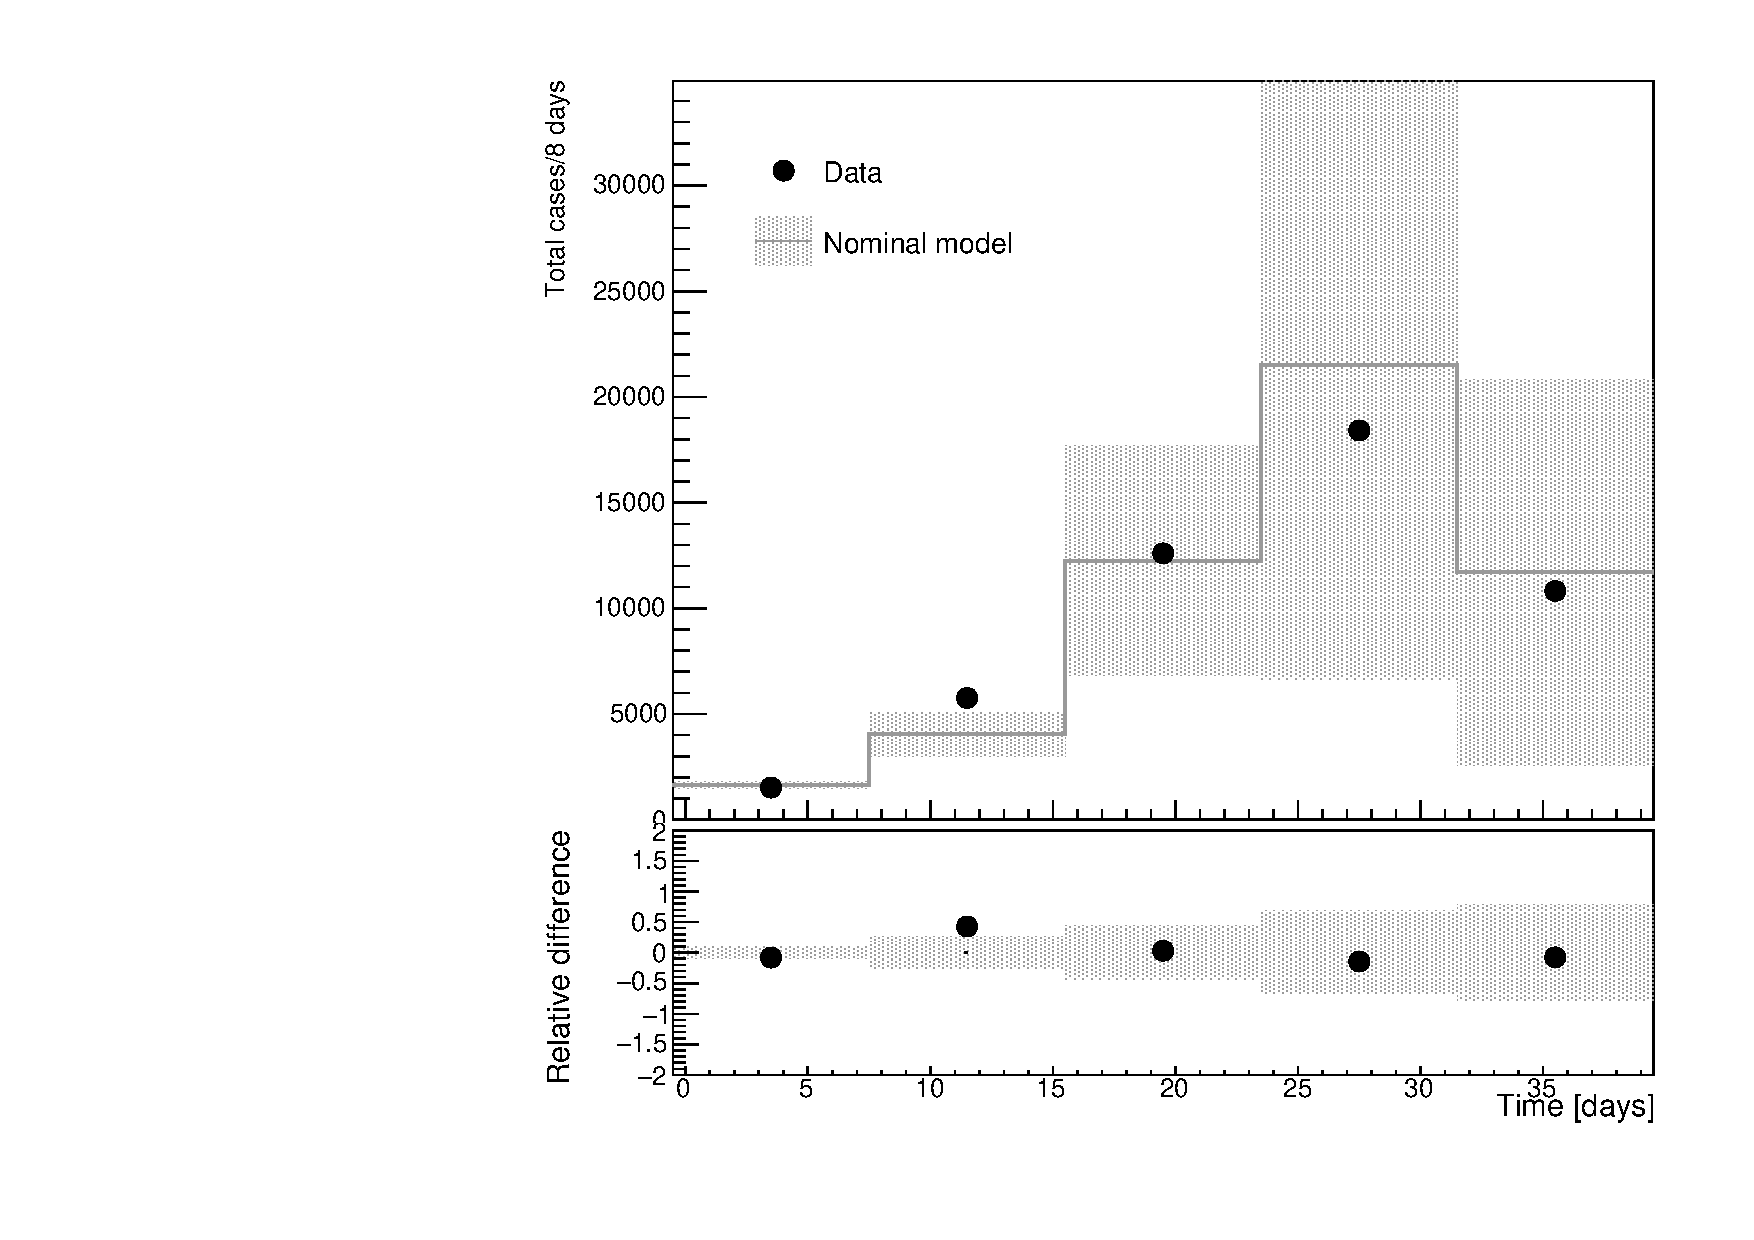
\includegraphics[width=0.4\textwidth]{imgs/Covid/ModelPrefit.pdf} 
  \caption{Pre-fit prediction of the model with the corrections described in Figure~\ref{ssec:impr_model} and the parameters in Figure~\ref{fig:model_vs_time}. The total uncertainty is given by summing all the sources of uncertainties described in Section~\ref{ssec:plf}}
  \label{fig:prefit}
\end{figure}

\begin{figure}
\centering
\subfloat[]{ 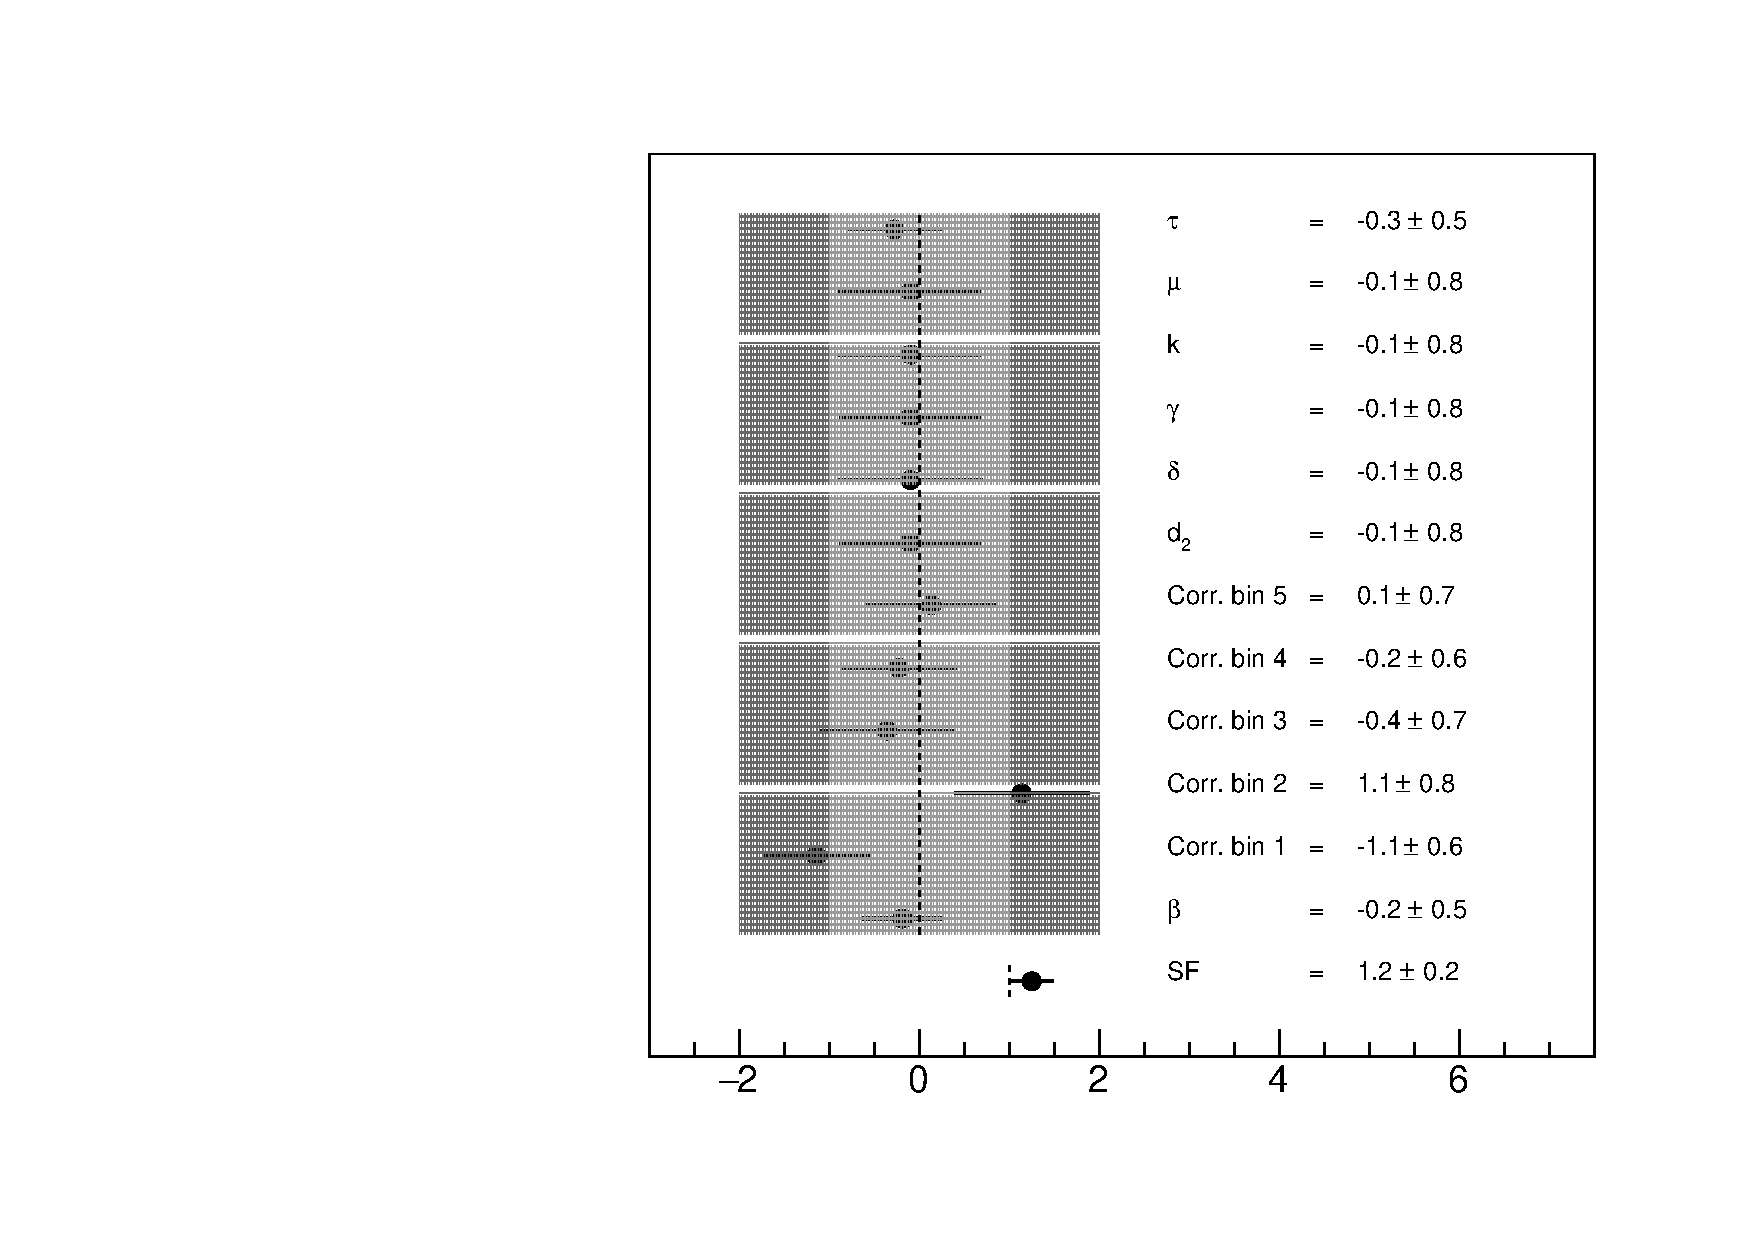
\includegraphics[width=0.45\textwidth]{imgs/Covid/PoI.pdf} }
\subfloat[]{ 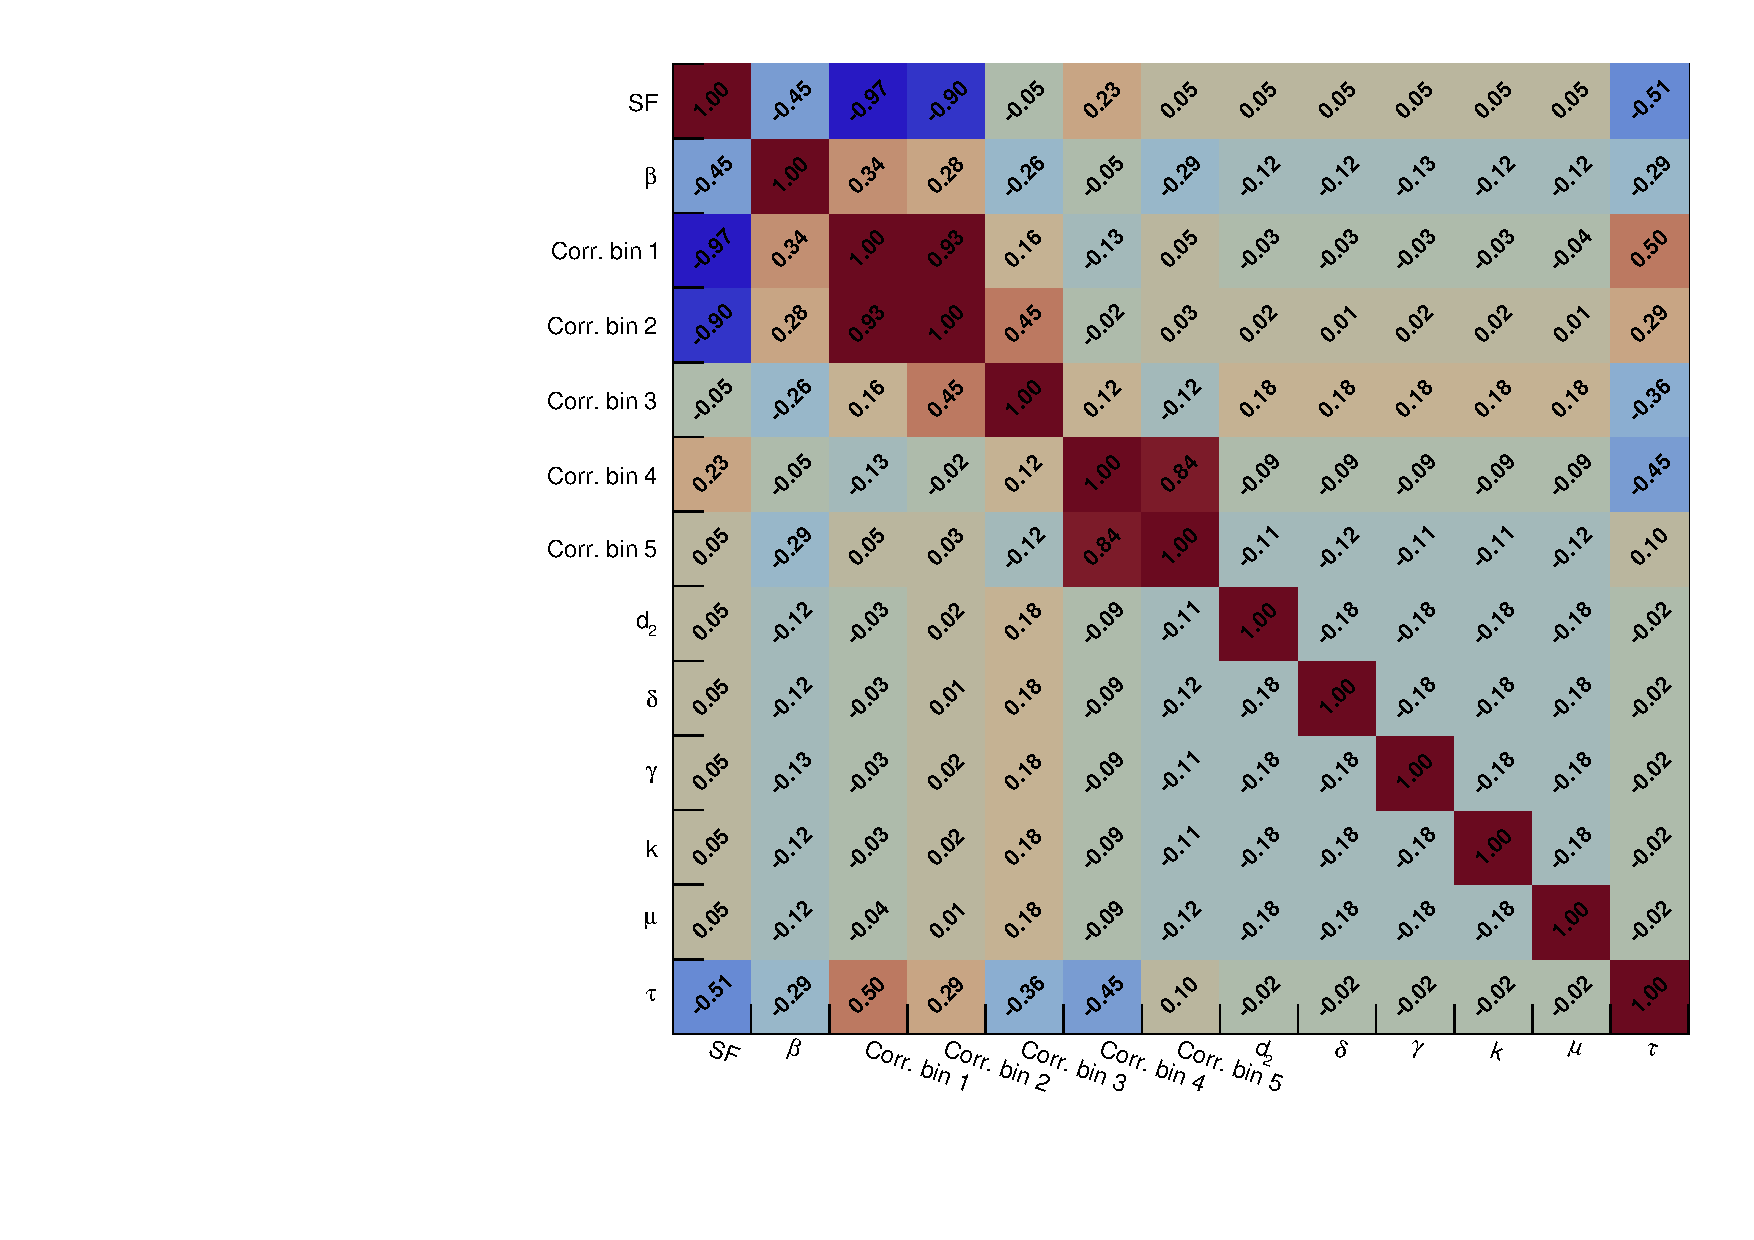
\includegraphics[width=0.4\textwidth]{imgs/Covid/CorrMatrix.pdf} }
  \caption{Fitted values of the model parameters (a). Correlations between the fitted parameters (b).}
  \label{fig:nps}
\end{figure}

The post-fit prediction is shown in Figure~\ref{fig:postfit}. The uncertainties are shrinked at higher bins, while enlarged in the lower bins because of the pulls and shows good agreement of the model with data within the fitted uncertainties.

\begin{figure}
\centering
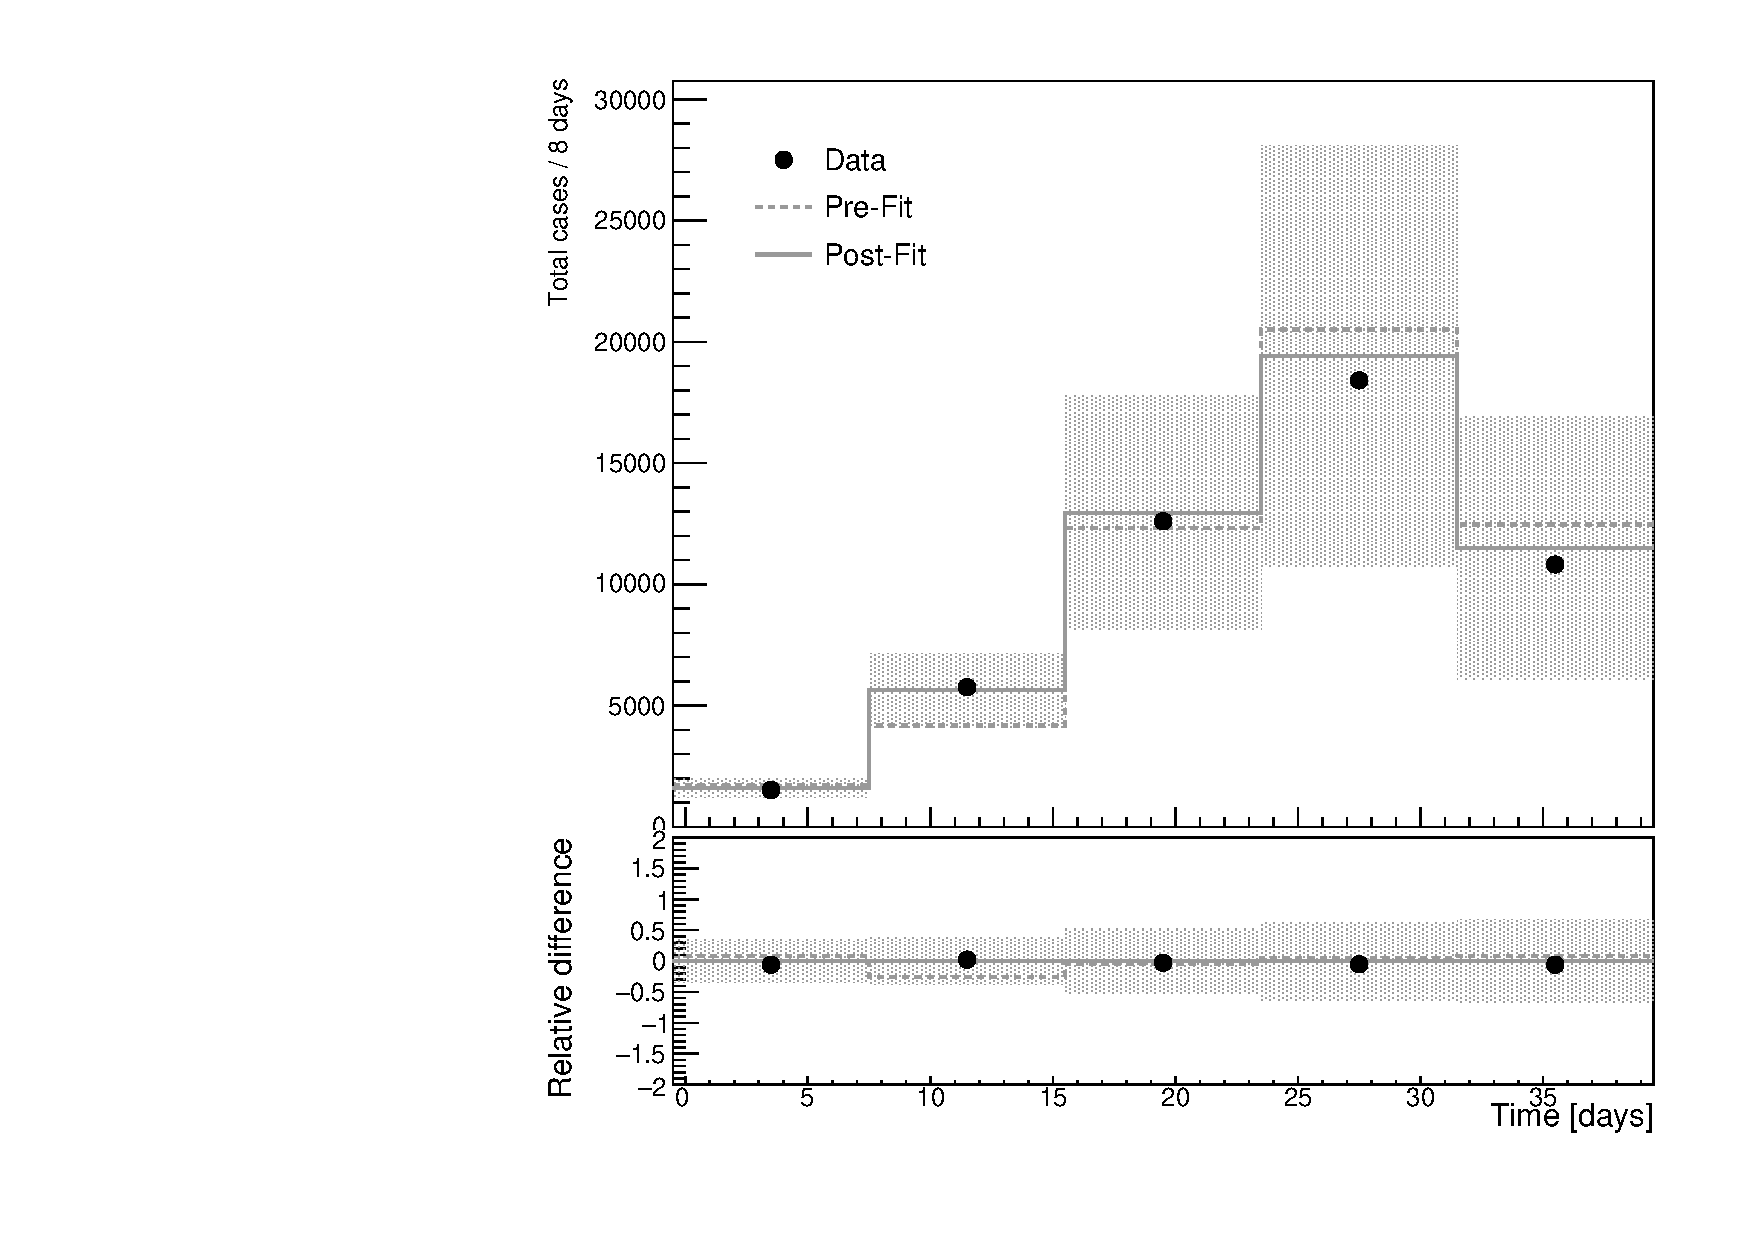
\includegraphics[width=0.4\textwidth]{imgs/Covid/ModelPostFit.pdf} 
  \caption{Post-fit prediction of the model with the corrections described in Figure~\ref{ssec:impr_model}, with parameters pulled as in Figure~\ref{fig:nps}a. The total uncertainty is given by summing all the post-fit uncertainties, correlated as in Figure~\ref{fig:nps}b.}
  \label{fig:postfit}
\end{figure}

\subsection{Predictions}
The fitted set of parameters is used to predict the evolution of the population categories evolutions, as shown in Figure~\ref{fig:model_postfit}a. In Figure~\ref{fig:model_postfit}b the evolution in time of $R_0$ is shown. $R_0$ stands for the infection power of each single individual. Here it is estimated as the ratio of the quarantined and infected (or just quarantined) population at time $t$ with the same quantity at time $t-\tau$, where $\tau $ is the incubation time. \\

\begin{figure}
\centering
\subfloat {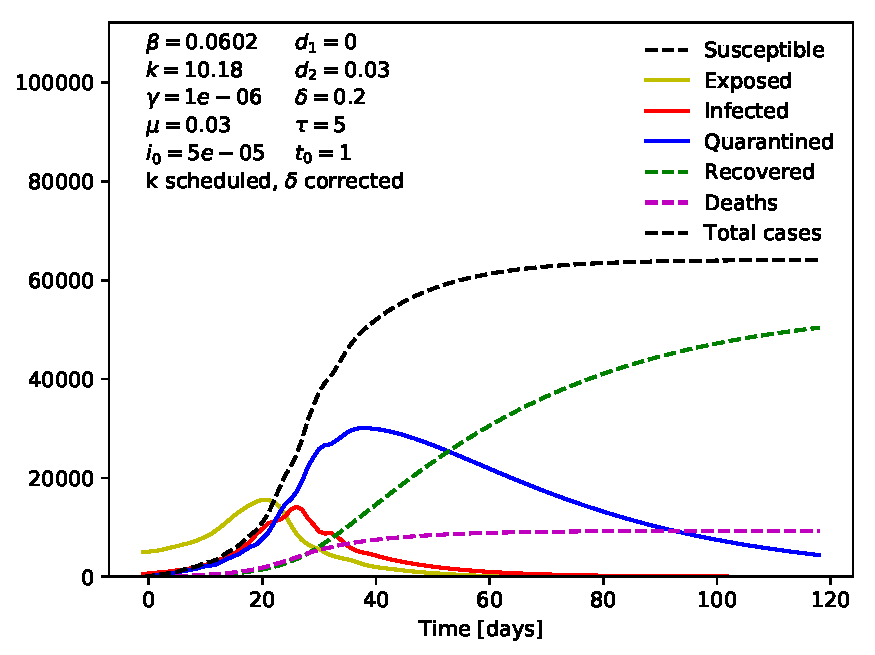
\includegraphics[width=0.4\textwidth]{imgs/Covid/Summary_parameters_Lombardia_scheduling_corrected_postfit_v2.pdf}  }
\subfloat {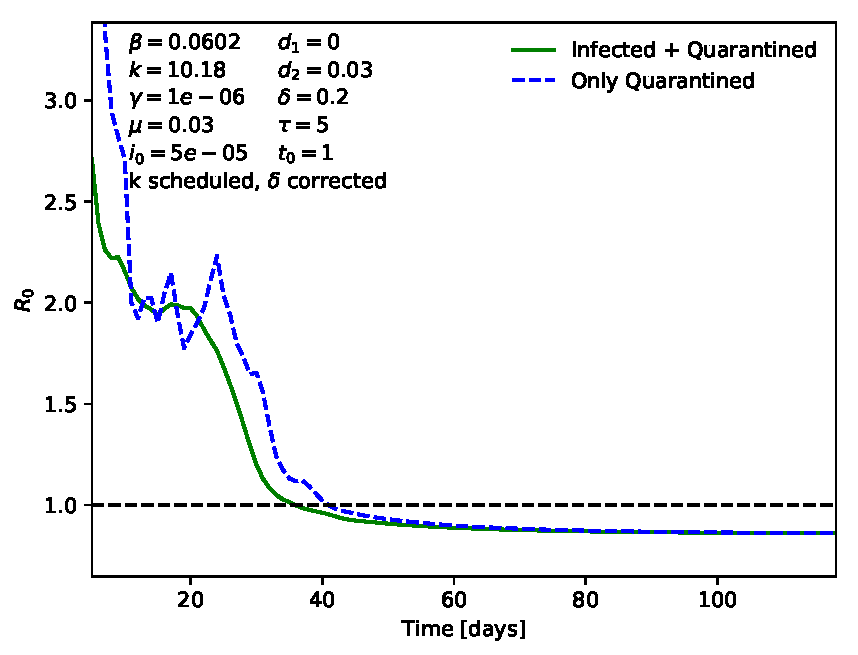
\includegraphics[width=0.4\textwidth]{imgs/Covid/R0_parameters_Lombardia_scheduling_corrected_postfit_v2.pdf}  }
  \caption{Prediction of the model tuned with the fitted parameters in Figure~\ref{fig:nps}a. Prediction of $R_0$ parameter against time (b).}
  \label{fig:model_postfit}
\end{figure}

The fitted model is used to predict some features of the virus spreading and to test them against the observations. To estimate the uncertainties on these estimations, a set of $1000$ pseudo-experiments is generated, obtained by extracting values of the model parameters from the fitted distributions, taking into account the fitted correlations. Predictions on a given observable are made by estimating mean and variance of the generated distribution from the pseudo-experiments. Since the fit is performed on the total cases distributions, predictions on the total cases related observables are more reliable. However, since quarantined population is the largest contribution to the total cases, especially in the fitted range, also the estimations of quarantined-related observables should be robust. The predictions on the number of deaths may be affected by the small contribution to the total cases in the fitted range, and therefore not very reliable. However, in the initial tuning (Figure~\ref{fig:model_vs_data}), the ratios between the contributions of the different classes is taken into account, so the obtained numbers should be in the same order of magnitude of the observations. A summary of the predictions on some observables of the outbreak evolution is given in Table~\ref{tab:predictions}.\\

\begin{table}\centering
\begin{tabular}{@{}lll@{}}
\toprule
Quantity & \phantom{abc} & Value \\
\midrule
\multicolumn{3}{@{}l@{}}{\emph{Quarantined people}}\\[1mm]
Peak & \phantom{abc} & $ 36000 \pm 21000 $\\
Peak time & \phantom{abc} & $ 38\pm1 $ days\\[3mm]

\multicolumn{3}{@{}l@{}}{\emph{Deaths}}\\[1mm]
Total deaths & \phantom{abc} & $ 13000 \pm 9000 $\\[3mm]

\multicolumn{3}{@{}l@{}}{\emph{Total cases}}\\[1mm]
Total & \phantom{abc} & $ 88000 \pm 67000 $\\
Saturation time & \phantom{abc} & $ 56\pm7 $ days\\
\bottomrule
\end{tabular}
\caption{Predictions of the model on some observables of the outbreak. The model is tuned with the fitted parameters in Figure~\ref{fig:nps}a. Dates are expressed in days after February 27th, the first day of available data.}
  \label{tab:predictions}
\end{table}

Currently (on 16/04/2020), from the updated data on reference \cite{Lab24}, there are $62153$ total cases, with $11377$ deaths. Both numbers are compatible with the predictions within the large uncertainties, but at least in the correct order of magnitude. The model predicts the peak of quarantined (positive) cases on April 2nd, however not a simple comparison with data is possible due to a lack of data documentation. The observed peak of daily new total cases is observed between March 21st and 26th, 2020: this is the highest slope of the total cases distribution against time, so expected earlier than the peak of quarantined population. A first decrease of total intensive in Italy care has been observed on April 4th, withing 2 standard deviations from the expectation. A comparison in terms of $R_0$ parameter is also possible.  The $R_0$ evolution, shown in Figure~\ref{fig:model_postfit}, can be tested as well. Considering the $R_0$ estimated only using quarantined population yields, an $R_0<1$ occurs around the 42th day, so on April 6th. The first indication of a $R_0<1$ in Italy is reported on April 9th \cite{R0}, quite close to the expectations. Unfortunately both  previous data are available only national-wise and not for Lombardy only, so results may differ. Finally, the estimated time of saturation of the total cases, corresponding to  reaching the $90\%$ of the maximum total cases, is expected in the week around April 20th.\\



